\chapter{Теоретическое обоснование разработанного алгоритма}
\label{chapter2}

В данной главе будут представлены теоретические результаты работы, а именно описана схема создания гибридного алгоритма, приведены требования от кандидатов на роль основных алгоритмов, описан новый алгоритм недоминирующей сортировки, который далее используется для создания гибридного алгоритма. 

\section{Анализ существующих алгоритмов}

Основным кандидатом для создания гибридного алгоритма недоминирующей сортировки оказался алгоритм Буздалова и др. на основе метода ``разделяй и властвуй''. Есть две основные причины, чтобы использовать этот алгоритм:

\begin{enumerate}
 \item Данный алгоритм основан на методе ``разделяй и властвуй'', что позволяет использовать рекурсивные вызовы к качестве точек подключения с одного алгоритма на другой.
 \item Данный алгоритм является одним из лучших алгоритма на сегодняшний день, и имеет доказанную, хорошую асимптотику времени работы.
\end{enumerate}

Вторым кандидатом стал алгоритм Роя, который уже показал неплохие результаты в гибриде с алгоритмом Буздалова \cite{Markina}, но алгоритм Роя был только наполовину приспособлен для гибридизации. В этой работе представлена попытка приспособить его полностью. 

Третьим кандидатом стал алгоритм Густавссона ENS-NDT, использование которого для создания гибридного алгоритма сильно снизило эффективность гибридного алгоритма недоминирующей сортировки. Вдохновившись идеями алгоритма Густавссона, мы получили новый алгоритм и назвали его ENS-NDT-ONE. Сам по себе он уже имеет некоторый научный интерес, так как имеет хорошую асимптотику и эффективен на практике наравне с лучшими алгоритмами недоминирующей сортировки. Затем мы реализовали гибридный алгоритм на основе алгоритма ``Разделяй и властвуй'' и алгоритма ENS-NDT-ONE.

\section{Предлагаемая схема гибридного алгоритма}

В этом разделе будет описана предлагаемая схема гибридного алгоритма.

\subsection{Выбор момент переключения}

Алгоритм ``разделяй и властвуй'' очень хорошо подходит для создания гибридного алгоритма недоминирующей сортировки, так как в алгоритме рекурсивно вызываются подзадачи меньшего размера и меньшей размерности. В первой главе данной работы описан алгоритм подробно, в оригинальной статье функции, где мы предполагаем переключаться на другой алгоритм, названы $HeplerA$ и $HeplerB$. Мы предлагаем следующую идею создания гибридного алгоритма: 
\begin{enumerate}
  \item Запускаем алгоритм Divide\&Conquer, согласно некоторым правилам переключаемся на другой алгоритм.
  \item Моменты смены алгоритма:
    \begin{enumerate}
    \item HelperA
      \begin{enumerate}
      \item Входные данные: множество точек $S$ с предварительными рангами.
      \item Результат выполнения: множество точек $S$ с обновленными рангами.
      \end{enumerate}
    \item HelperB  
      \begin{enumerate}
      \item Входные данные: множество точек $L$ с окончательными рангами и $R$ с предварительными рангами.
      \item Результат выполнения: множество точек $R$ с обновленными рангами по множеству $L$.
      \end{enumerate}
    \end{enumerate}
\end{enumerate}

\subsection{Настройка параметров гибридизации}

Настройка гибридного алгоритма будет представлять некоторый диапазон размеров множестве точек для каждой размерности, при котором происходит переключение. Например, при размерности точек три, договоримся, что смена алгоритма происходит если точек не больше 100, а при размерности 4 и более смена происходит при размере множеств точек не более 1000. Параметры гибридизации получаются экспериментальным путем для конкретного вида гибридного алгоритма. Параметры, полученные в данной работе, описаны в разделе 3.3.

\section{Адаптация алгоритмов}

В этом разделе опишем адаптацию алгоритмов для гибридизации. Для гибридизации было выбрано два алгоритма: алгоритм Роя и алгоритм Густавссона. Идеи гибридизации и адаптации схожи, поэтому опишем их сначала в общем случае, потом перейдем к деталям каждого алгоритма. 

Функция $HeplperA$ {---} это сама недоминирующая сортировка, поэтому приспосабливать алгоритмы с этой точки зрения не надо.

Напомним, что функция $HeplerB$ в качестве входных параметров принимала два множества $L$ с окончательными рангами и $R$ с предварительными рангами, по результату работы назначаются ранги множеству точек $R$ по множеству точек $L$. 

Для $HeplerB$ была предложена следующая идея адаптации для гибридизации: 
\begin{enumerate}
  \item Обходим точки в порядке предложенном в оригинальном алгоритме.
  \begin{enumerate}
      \item Если точка принадлежит множеству с окончательными рангами $L$, добавляем точку в структуру алгоритма с текущим рангом.
      \item Если точка принадлежит множеству с предварительными рангами $R$, то мы определяем ранг рассматриваемой точки на основе текущего состояния структуры и не добавляем ее в структуру, так как ранжирование происходить только на основе точек из множества $L$.
  \end{enumerate}
\end{enumerate}


Основные отличия от оригинального алгоритма: 
\begin{enumerate}
    \item В оригинальной статье на момент начала работы алгоритма все точки имели ранг 0, в нашем случае начальные ранги могут быть любыми.
    \item Определение ранга точек надо изменить, чтобы алгоритм учитывал предпоставленные ранги.
\end{enumerate}

Рассмотрим отдельно для каждого алгоритма адаптацию для последующей реализации гибридного алгоритма.

\subsection{Алгоритм Роя и др.}

Алгоритм предложенный Роем и др. описан подробно в главе Обзор работы. Ранее был предложен гибридный алгоритм, который использует только момент переключения $HelperA$ \cite{Markina}, второй момент переключения $HelperB$ не был рассмотрен в данной работе. 

Определение ранга происходило бинарным или последовательным поиском с нулевого ранга по ранжированному множеству точек. Эффективность этих двух подходов практически совпадала. Найденное множество точек с минимальным рангом, где ни одна точка не доминирует рассматриваемую, означало, что точке можно присвоить ранг этого множества. Был справедлив следующий инвариант: для рассматриваемой точки до некоторого ранга $k$ все множества соответствующие меньшим $k$ рангам имеют хотя бы одну точку, которая доминирует рассматриваемую, а начиная с множества соответствующего рангу $k$ и больше во всех множествах нет ни одной точки, которая бы доминировала рассматриваемую точку. В таком случае точка получает ранг $k$. 

В новой версии алгоритма в множестве $L$, точки которого добавляются в структуру позволяющую определять ранг, могут иметь совершенно любые ранги. И точка может доминироваться точкой, например, ранга $k$, но не доминироваться точкой $k-1$ ранга, это означает, что больше нельзя использовать бинарный поиск для определения ранга. Единственным выходом является перебор множеств начиная с наибольшего в структуре, пока не найдется множество, где есть хотя бы одна точка, которая доминирует рассматриваемую. После этого можно сделать вывод, что точка имеет ранг найденного множества + 1. 

После такого значительного изменения алгоритма мы провели замеры времени работы и оказалось, что новый алгоритм работает на порядок хуже оригинального алгоритма, это означает, что создать гибридный алгоритм на его основе нельзя, по крайней мере используя такой подход гибридизации. Теоретическое исследование времени алгоритма является достаточно трудоемкой задачей и из-за настолько плохого практического результата, мы не стали им заниматься. 

\subsection{Алгоритм Густавссона и др.}

Следующим кандидатом для гибридизации был алгоритм Густавссона и др. 

Время работы этого алгоритма на случайно сгенерированных, независимых точках в гиперкубе составляет $O(N^{1.43})$, но авторами работы описан худший случай, на котором асимптотика становится квадратичной и составляет $O(MN^2)$, на больших N время работы становится неприемлемо большим. Алгоритм выбран в качестве основного кандидата для гибридизации, потому что он является самым эффективным алгоритмом на сегодняшний день в общем случае. 

\section{Новый алгоритм ENS-NDT-ONE}

В данном разделе опишем новый алгоритм ENS-NDT-ONE и представим асимптотическую оценку времени работы.

\subsection{Причины необходимости нового алгоритма}

В оригинальном алгоритме точки, которые необходимо отсортировать, инициировались рангом $0$, и ранг назначался постепенно, в лексикографическом порядке. Теперь точки в качестве аргументов приходят в алгоритм Густавссона из базового алгоритма Буздалова. Точки могут иметь совершенно разные ранги, в том числе для конкретной рассматриваемой точки, может оказаться, что ни одна точки с рангом $0$, ее не доминирует, что раньше бы привело, к присвоениею этой точки ранга $0$, а точка с рангом больше $0$ доминирует. То есть определение ранга происходило похожим на алгоритм Роя образом, присутствовала монотонность, то есть первое найденное множество с минимальным рангом, где ни одна точка не доминирует рассматриваемую, означает, что точке можно присвоить ранг этого множества. В структуре недоминирующих деревьев, где каждое дерево соответствует своему рангу, мы бинарным поиском определяли минимально по рангу дерево, где, аналогично, ни одна точка не доминирует рассматриваемую, тогда рассматриваемой точке присваивался ранг этого дерева. Но аналогично проблеме описанной выше, в алгоритме Роя, инвариант позволяющий осуществить бинарный поиск перестает работать. Теперь надо искать точку с максимальным рангом, которая доминирует рассматриваемую. Тогда точке, для которой производится определение ранга, назначается ранг найденной точки $+ 1$.  

Таким образом, алгоритм был адаптирован следующим образом: вместо бинарного поиска использовался последовательный перебор с дерева, соответствующего максимальному рангу, переходя к деревьям меньшего ранга. После этого, мы провели эмпирический анализ времени работы, который показал, что потеря монотонности, критически влияет на время работы. Теоретический анализ адаптированного алгоритма не был произведен, из-за плохого практического результата.

Описанные выше изменения вдохновили на создание нового алгоритма на основе недоминирующего дерева, на которое отсутствие монотонности не производило бы такого сильного замедления. Новый алгоритм был назван ENS-NDT-ONE.

\subsection{Описание алгоритма}

Алгоритм ENS-NDT был изменен следующим образом: вместо множества деревьев теперь будем хранить одно дерево для всех точек, именно по этой причине, алгоритм назван ENS-NDT-ONE. Параметрами дерева, как в оригинальной версии алгоритма, будет размер корзины, ограничивающий максимальное количество точек, которое может содержаться в одной вершине, и вторым параметром будет глубина, начиная с которой размер корзины игнорируется, и точки перестают делиться на две при превышении первого порога. Так же как в оригинальном алгоритме дерево будет сбалансированным, это обеспечивается предварительно подсчитанной структурой $split$. На рисунке ~\ref{ndtree_new} представлено схематическое представление алгоритма ENS-NDT-ONE.

\begin{figure}[!h]
\begin{center}
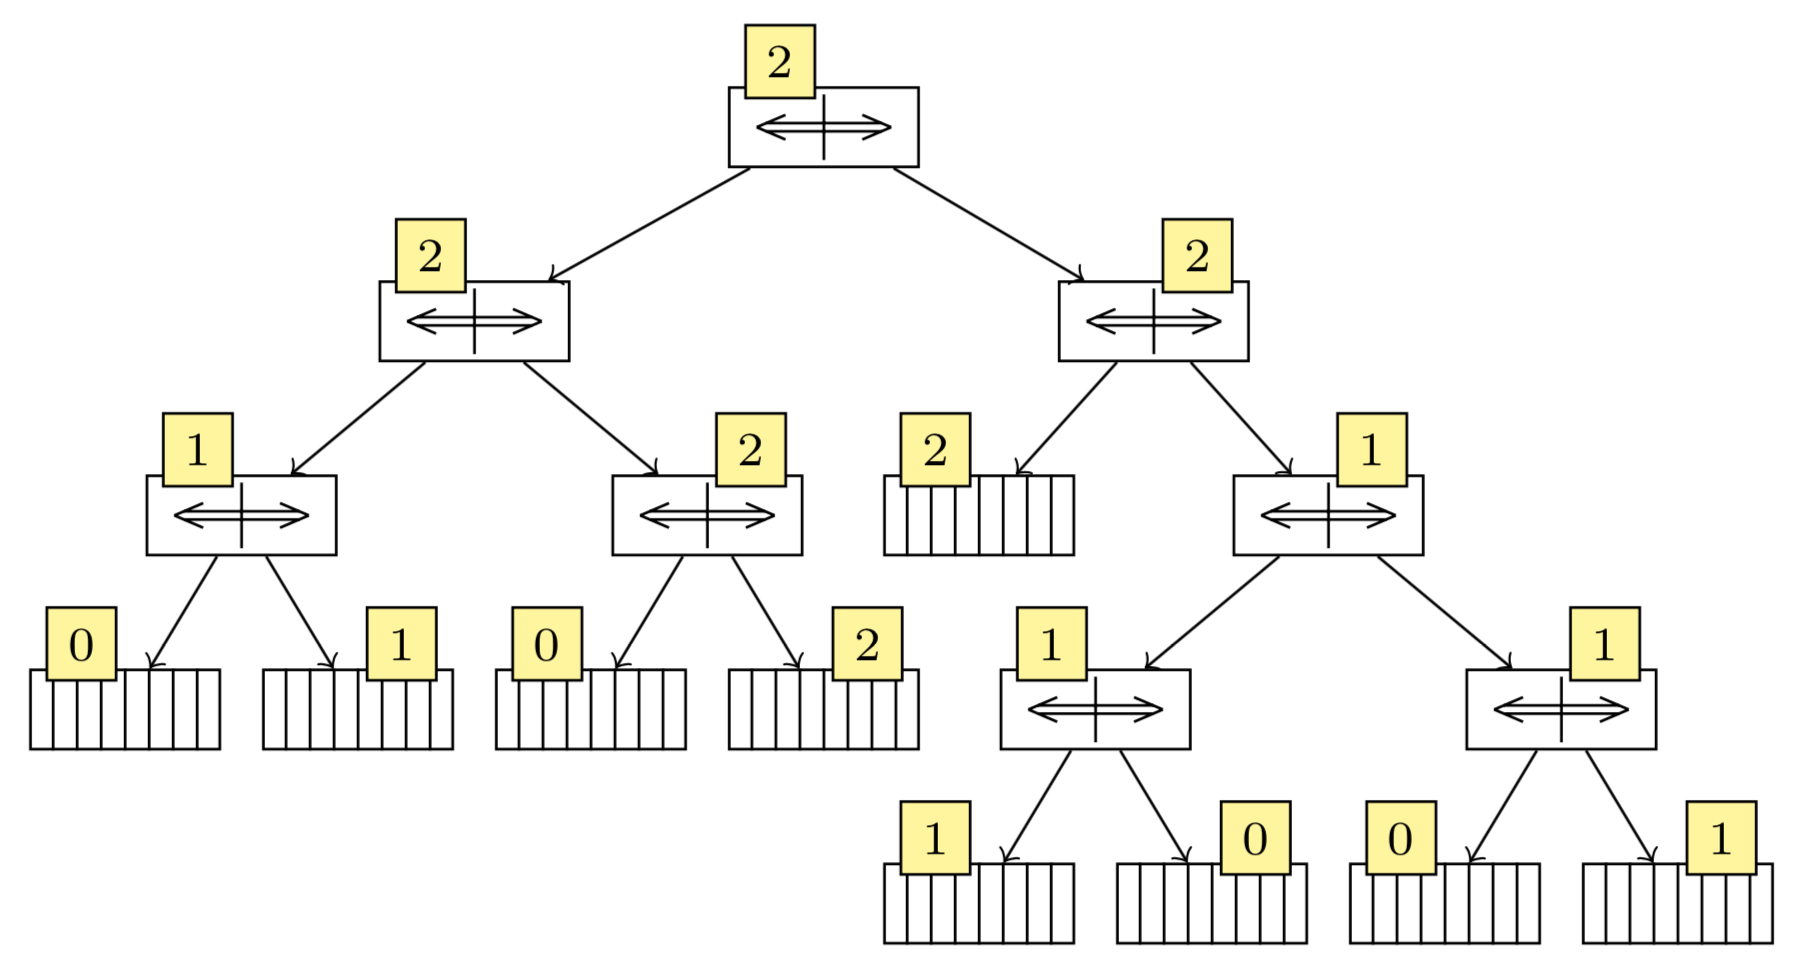
\includegraphics[width=15cm]{pic/ndtree_new.png}
\caption{Алгоритм ENS-NDT-ONE}.
\label{ndtree_new}
\end{center}
\end{figure}

Одним из преимуществ производительности алгоритма ENS-NDT было то, что, выполняя определение ранга для точки $p$ в некотором дереве, как только найденная точка доминирующая точку $p$, можно сразу же закрыть это дерево, так как больше точек из этого дерева не может влиять на ранг $p$. Это не так для алгоритма ENS-NDT-ONE, так как в дереве могут встретиться точки с большим или равным раном, чем ранг рассматриваемой точки $p$.

Чтобы предотвратить потери производительности, мы предлагаем хранить максимальный ранг всех точек на поддереве. Это позволит при определении точки с изначальным рангом $k$, не спускаться в поддерево с рангом $\leq k$. На фазе добавления точки в дерево необходимо не забыть обновить значения максимального ранга по пути добавления.

Адаптация для функции $HeplerA$ не требуется, так как это обычная недоминирующая сортировка. При обновлении ранга надо только учитывать предварительный ранг точки, и обновлять ранг только в том случае, если он был меньше, чем новый ранг. Напомним, что процедура $HeplerB$ принимает в качестве аргументов два множества, одно с окончательными рангами $L$, другое предварительными рангами $R$. В процедуре $HeplerB$ происходит обновление рангов множества $R$, по рангам множества $L$. Опишем работу алгоритма ENS-NDT-ONE с двумя множествами $L$ и $R$: 
\begin{enumerate}
  \item Обходим точки в лексикографическом порядке, как в оригинальном алгоритме.
  \begin{enumerate}
      \item Если точка принадлежит множеству с окончательными рангами $L$, добавляем точку в дерево с текущим рангом.
      \item Если точка принадлежит множеству с предварительными рангами $R$, то мы обновляем ранг рассматриваемой точки по дереву и не добавляем ее в структуру, так как ранжирование происходить только на основе точек из множества $L$.
  \end{enumerate}
\end{enumerate}

\subsection{Асимптотика времени работы}

Вероятность пропуска поддеревьев сильно влияет на производительность алгоритма ENS-NDT-ONE. В частности, для многих видов входных точек можно показать постоянную верхнюю границу $\alpha$ на вероятность входа в дочерний узел, который соответствует более высокому значению по критерию, рассматриваемому на данном слое. Из этого получаем верхнюю границу $O(MN^{\log_2(1+\alpha)})$ на один запрос и $O(MN^{1+\log_2(1+\alpha)})$ для всей сортировки, что строго быстрее, чем $\Theta(N^2M)$, когда $\alpha<1$. В худшем случае алгоритм ENS-NDT-ONE работает за $O(MN^2)$, однако зачастую время работы алгоритма сильно лучше. Например, на случайно сгенерированных точках в гиперкубе $[0; 1]^M$, $O(N)$ точек с вероятностью не более $1/2$ необходимо заходить в обоих детей в каждой не листовой вершине дерева. Таким образом получаем, что верхняя граница асимптотики времени работы равна $O(MN^{1+\log_2(1+1/2)}) \approx O(MN^{1.585})$.

\section{Гибридный алгоритм}

\subsection{Формулировка гибридного алгоритма}

Теперь мы можем сформулировать гибридный алгоритм. Мы используем алгоритм ``разделяй и властвуй'' как базовый алгоритм, каждый раз прежде чем вызывать процедуры $HelperA$ и $HelperB$, мы проверяем размер точек, на которых необходимо выполнить сортировку. Если точки с таким размером эффективно сортируются в алгоритме ENS-NDT-ONE, переключается с базового алгоритма на алгоритм ENS-NDT-ONE для решения этой подзадачи. Так как алгоритм приспособлен к гибридизации, в том числе невосприимчив к отсутствию монотонности, и учитывает предпоставленные ранги в базовом алгоритме, полученный алгоритм будет работать корректно.

Если говорить более формально, мы определяем для каждого значения размерности пороговое значение, которое означает, что каждая подзадача с таким и меньшим размером точек должна быть делегирована алгоритму ENS-NDT-ONE. Для процедуры $HelperA$ размер множества точек {---} это размер множества $S$, для процедуры $HelperB$ {---} это сумма размеров множеств $L$ и $R$.

\subsection{Анализ времени работы гибридного алгоритма}

В этом разделе дадим некоторую оценку асимптотики времени работы гибридного алгоритма.

Напомним, что время работы алгоритма Буздалова асимптотически равно $O(N(\log N)^{M-1})$. Так как мы определяем пороговые значения как константы, асимптотическая оценка времени работы итогового гибридного  алгоритма по-прежнему равна $O(N(\log N)^{M-1})$. Заметим, что тщательный выбор пороговых значений, например, добавить зависимость от вида входных данных, может улучшить асимптотическую оценку. Так как эта задача является сложной, мы оставляем это для возможной будущей работы.

